% Options for packages loaded elsewhere
\PassOptionsToPackage{unicode}{hyperref}
\PassOptionsToPackage{hyphens}{url}
%
\documentclass[
]{article}
\usepackage{lmodern}
\usepackage{amssymb,amsmath}
\usepackage{ifxetex,ifluatex}
\ifnum 0\ifxetex 1\fi\ifluatex 1\fi=0 % if pdftex
  \usepackage[T1]{fontenc}
  \usepackage[utf8]{inputenc}
  \usepackage{textcomp} % provide euro and other symbols
\else % if luatex or xetex
  \usepackage{unicode-math}
  \defaultfontfeatures{Scale=MatchLowercase}
  \defaultfontfeatures[\rmfamily]{Ligatures=TeX,Scale=1}
\fi
% Use upquote if available, for straight quotes in verbatim environments
\IfFileExists{upquote.sty}{\usepackage{upquote}}{}
\IfFileExists{microtype.sty}{% use microtype if available
  \usepackage[]{microtype}
  \UseMicrotypeSet[protrusion]{basicmath} % disable protrusion for tt fonts
}{}
\makeatletter
\@ifundefined{KOMAClassName}{% if non-KOMA class
  \IfFileExists{parskip.sty}{%
    \usepackage{parskip}
  }{% else
    \setlength{\parindent}{0pt}
    \setlength{\parskip}{6pt plus 2pt minus 1pt}}
}{% if KOMA class
  \KOMAoptions{parskip=half}}
\makeatother
\usepackage{xcolor}
\IfFileExists{xurl.sty}{\usepackage{xurl}}{} % add URL line breaks if available
\IfFileExists{bookmark.sty}{\usepackage{bookmark}}{\usepackage{hyperref}}
\hypersetup{
  pdftitle={Taller 1: Análisis Multivariado},
  pdfauthor={Julián Camilo Riaño Moreno},
  hidelinks,
  pdfcreator={LaTeX via pandoc}}
\urlstyle{same} % disable monospaced font for URLs
\usepackage[margin=1in]{geometry}
\usepackage{longtable,booktabs}
% Correct order of tables after \paragraph or \subparagraph
\usepackage{etoolbox}
\makeatletter
\patchcmd\longtable{\par}{\if@noskipsec\mbox{}\fi\par}{}{}
\makeatother
% Allow footnotes in longtable head/foot
\IfFileExists{footnotehyper.sty}{\usepackage{footnotehyper}}{\usepackage{footnote}}
\makesavenoteenv{longtable}
\usepackage{graphicx,grffile}
\makeatletter
\def\maxwidth{\ifdim\Gin@nat@width>\linewidth\linewidth\else\Gin@nat@width\fi}
\def\maxheight{\ifdim\Gin@nat@height>\textheight\textheight\else\Gin@nat@height\fi}
\makeatother
% Scale images if necessary, so that they will not overflow the page
% margins by default, and it is still possible to overwrite the defaults
% using explicit options in \includegraphics[width, height, ...]{}
\setkeys{Gin}{width=\maxwidth,height=\maxheight,keepaspectratio}
% Set default figure placement to htbp
\makeatletter
\def\fps@figure{htbp}
\makeatother
\setlength{\emergencystretch}{3em} % prevent overfull lines
\providecommand{\tightlist}{%
  \setlength{\itemsep}{0pt}\setlength{\parskip}{0pt}}
\setcounter{secnumdepth}{-\maxdimen} % remove section numbering
\usepackage{float}
\floatplacement{figure}{H}
\usepackage{booktabs}
\usepackage{longtable}
\usepackage{array}
\usepackage{multirow}
\usepackage{wrapfig}
\usepackage{float}
\usepackage{colortbl}
\usepackage{pdflscape}
\usepackage{tabu}
\usepackage{threeparttable}
\usepackage{threeparttablex}
\usepackage[normalem]{ulem}
\usepackage{makecell}
\usepackage{xcolor}

\title{Taller 1: Análisis Multivariado}
\usepackage{etoolbox}
\makeatletter
\providecommand{\subtitle}[1]{% add subtitle to \maketitle
  \apptocmd{\@title}{\par {\large #1 \par}}{}{}
}
\makeatother
\subtitle{Introducción y graficas para el análisis mulivariado}
\author{Julián Camilo Riaño Moreno}
\date{jueves, junio 18, 2020}

\begin{document}
\maketitle

{
\setcounter{tocdepth}{3}
\tableofcontents
}
\hypertarget{actividad-1}{%
\subsection{Actividad \#1}\label{actividad-1}}

\begin{quote}
Busque un conjunto de datos multivariados relacionados con un área de
conocimiento de su dominio que tenga al menos 50 observaciones, 5
variables numéricas y 3 categóricas.
\end{quote}

\hypertarget{especificaciones-sobre-la-base-de-datos-utilizada.}{%
\subsection{Especificaciones sobre la base de datos
utilizada.}\label{especificaciones-sobre-la-base-de-datos-utilizada.}}

Para la elaboración de las actividades propuestas en el curso de
análisis multivariado, se decidió utiliza una base de datos que se desea
utilizar para un trabajo de investigación en marco de la
\emph{especialización en estadística aplicada}.

Los datos para estos análisis son obtendios de la iniciativa \emph{Data
from the ECDC Surveillance Atlas} para seguimiento de la resistencia a
antibióticos en la unión europea llevado acabo por el \emph{European
Centre for Disease Prevention and Control}. Esta información se puede
descargar desde el siguiente link:
(\url{https://atlas.ecdc.europa.eu/public/index.aspx?Dataset=27\&HealthTopic=4}).

La base de datos original cuenta con 67542 observaciones y 9 variables
(\emph{HealthTopic; Population; Indicator; Unit; Time; RegionCode;
RegionName; NumValue; TxtValue}).

A través de una limpieza exhaustiva y reorganización de esta base de
datos, se llegó a obtener una base de datos de 3478 observaciones y 72
variables, estas 72 variables corresponde a al tipo de \emph{Indicador}
por \emph{Antibiótico}, por ejemplo: nombre de la columna o variable
\emph{Vancomycin\_r\_percentage}, esto corresponde al porcentaje de
resistencia a la vancomicina. Estas variables son para cara cada una de
las 8 bacterias reportadas en el informe (\emph{Acinetobacter spp;
Enterococcus faecalis; Enterococcus faecium; Escherichia coli;
Klebsiella pneumoniae; Pseudomonas aeruginosa; Staphylococcus aureus;
Streptococcus pneumoniae}) y para los 30 países involucrados
(\emph{Austria, Belgium, Bulgaria, Croatia, Cyprus, Czechia, Denmark,
Estonia, Finland, France, Germany, Greece, Hungary, Iceland, Ireland,
Italy, Latvia, Lithuania, Luxembourg, Malta, Netherlands, Norway,
Poland, Portugal, Romania, Slovakia, Slovenia, Spain, Sweden, United
Kingdom}); esta información ha sido recolectada en los años 2000 - 2018.

Se realizó un reanálisis de la base de datos, se eliminaron las
variables que no eran informativas como por ejemplo las que se referían
al número de aislados en cada una de estas; se eliminaron sin
información (\emph{NAs}); únicamente se dejaron las variables que
correspondían al \% de resistencia para cada uno de los antibióticos
reportados para cada una de las bacterias\footnote{para tratar cada
  bacteria se utilizan diferentes antibióticos, de manera que los \% de
  resistencia reportados en esta base de datosn son algunos diferentes
  (algunos son los mismos) entre bacterias.}.

A continuación, se decidió seleccionar únicamente dos bacterias en las
que fueron evaluados los perfiles de resistencia a los mismos
antibióticos, a saber: Escherichia coli; Klebsiella pneumoniae. Las
cuales además registran los mayores números de observaciones (después de
la remoción de \emph{NAs}), 460 y 384 respectivamente. La variables de
esta nueva base de datos son : Bacteria, Year, Code\_C, Country,
Aminoglycosides, Carbapenems, Fluoroquinolones, cephalos\_3er\_gen.

Adicionalmente se realizón un \emph{web scrapping} de la página:
(`\url{https://www.worldatlas.com/articles/the-four-european-regions-as-defined-by-the-united-nations-geoscheme-for-europe.html}'),
para obtener las regiones del continente europeo al que corresponde del
que se obtuvieron observaciones. Se realizó un \emph{match} por la
variable \texttt{Country} y se adicionó una nueva variable llamada
\texttt{Region} a la base de datos final. Las especificaciones de las
variables de la base datos final se encuentran en la tabla 1.

\begin{longtable}[]{@{}ccccc@{}}
\caption{Organizacion de las variables de la base de
datos}\tabularnewline
\toprule
\begin{minipage}[b]{0.16\columnwidth}\centering
Nombre de variable\strut
\end{minipage} & \begin{minipage}[b]{0.21\columnwidth}\centering
Definicion\strut
\end{minipage} & \begin{minipage}[b]{0.24\columnwidth}\centering
Descripción\strut
\end{minipage} & \begin{minipage}[b]{0.07\columnwidth}\centering
Unidad\strut
\end{minipage} & \begin{minipage}[b]{0.18\columnwidth}\centering
Tipo de variable\strut
\end{minipage}\tabularnewline
\midrule
\endfirsthead
\toprule
\begin{minipage}[b]{0.16\columnwidth}\centering
Nombre de variable\strut
\end{minipage} & \begin{minipage}[b]{0.21\columnwidth}\centering
Definicion\strut
\end{minipage} & \begin{minipage}[b]{0.24\columnwidth}\centering
Descripción\strut
\end{minipage} & \begin{minipage}[b]{0.07\columnwidth}\centering
Unidad\strut
\end{minipage} & \begin{minipage}[b]{0.18\columnwidth}\centering
Tipo de variable\strut
\end{minipage}\tabularnewline
\midrule
\endhead
\begin{minipage}[t]{0.16\columnwidth}\centering
Bacteria\strut
\end{minipage} & \begin{minipage}[t]{0.21\columnwidth}\centering
Especie de la bacteria\strut
\end{minipage} & \begin{minipage}[t]{0.24\columnwidth}\centering
Escherichia coli o Klebsiella pneumoniae\strut
\end{minipage} & \begin{minipage}[t]{0.07\columnwidth}\centering
---\strut
\end{minipage} & \begin{minipage}[t]{0.18\columnwidth}\centering
Categorica nominal\strut
\end{minipage}\tabularnewline
\begin{minipage}[t]{0.16\columnwidth}\centering
Year\strut
\end{minipage} & \begin{minipage}[t]{0.21\columnwidth}\centering
Ano\strut
\end{minipage} & \begin{minipage}[t]{0.24\columnwidth}\centering
2000-2018\strut
\end{minipage} & \begin{minipage}[t]{0.07\columnwidth}\centering
Entero\strut
\end{minipage} & \begin{minipage}[t]{0.18\columnwidth}\centering
Categorica nominal\strut
\end{minipage}\tabularnewline
\begin{minipage}[t]{0.16\columnwidth}\centering
Code\_C\strut
\end{minipage} & \begin{minipage}[t]{0.21\columnwidth}\centering
Codigo del pais\strut
\end{minipage} & \begin{minipage}[t]{0.24\columnwidth}\centering
---\strut
\end{minipage} & \begin{minipage}[t]{0.07\columnwidth}\centering
---\strut
\end{minipage} & \begin{minipage}[t]{0.18\columnwidth}\centering
Categorica nominal\strut
\end{minipage}\tabularnewline
\begin{minipage}[t]{0.16\columnwidth}\centering
Country\strut
\end{minipage} & \begin{minipage}[t]{0.21\columnwidth}\centering
Nombre del pais\strut
\end{minipage} & \begin{minipage}[t]{0.24\columnwidth}\centering
---\strut
\end{minipage} & \begin{minipage}[t]{0.07\columnwidth}\centering
---\strut
\end{minipage} & \begin{minipage}[t]{0.18\columnwidth}\centering
Categorica nominal\strut
\end{minipage}\tabularnewline
\begin{minipage}[t]{0.16\columnwidth}\centering
Region\strut
\end{minipage} & \begin{minipage}[t]{0.21\columnwidth}\centering
Nombre de la region\strut
\end{minipage} & \begin{minipage}[t]{0.24\columnwidth}\centering
Eastern o Northern o Southern o Western\strut
\end{minipage} & \begin{minipage}[t]{0.07\columnwidth}\centering
---\strut
\end{minipage} & \begin{minipage}[t]{0.18\columnwidth}\centering
Categorica nominal\strut
\end{minipage}\tabularnewline
\begin{minipage}[t]{0.16\columnwidth}\centering
Aminoglycosides\strut
\end{minipage} & \begin{minipage}[t]{0.21\columnwidth}\centering
Porcentaje de resistencia\strut
\end{minipage} & \begin{minipage}[t]{0.24\columnwidth}\centering
---\strut
\end{minipage} & \begin{minipage}[t]{0.07\columnwidth}\centering
\%\strut
\end{minipage} & \begin{minipage}[t]{0.18\columnwidth}\centering
Cuantitativa continua\strut
\end{minipage}\tabularnewline
\begin{minipage}[t]{0.16\columnwidth}\centering
Carbapenems\strut
\end{minipage} & \begin{minipage}[t]{0.21\columnwidth}\centering
Porcentaje de resistencia\strut
\end{minipage} & \begin{minipage}[t]{0.24\columnwidth}\centering
---\strut
\end{minipage} & \begin{minipage}[t]{0.07\columnwidth}\centering
\%\strut
\end{minipage} & \begin{minipage}[t]{0.18\columnwidth}\centering
Cuantitativa continua\strut
\end{minipage}\tabularnewline
\begin{minipage}[t]{0.16\columnwidth}\centering
Fluoroquinolones\strut
\end{minipage} & \begin{minipage}[t]{0.21\columnwidth}\centering
Porcentaje de resistencia\strut
\end{minipage} & \begin{minipage}[t]{0.24\columnwidth}\centering
---\strut
\end{minipage} & \begin{minipage}[t]{0.07\columnwidth}\centering
\%\strut
\end{minipage} & \begin{minipage}[t]{0.18\columnwidth}\centering
Cuantitativa continua\strut
\end{minipage}\tabularnewline
\begin{minipage}[t]{0.16\columnwidth}\centering
cephalos\_3er\_gen\strut
\end{minipage} & \begin{minipage}[t]{0.21\columnwidth}\centering
Porcentaje de resistencia\strut
\end{minipage} & \begin{minipage}[t]{0.24\columnwidth}\centering
---\strut
\end{minipage} & \begin{minipage}[t]{0.07\columnwidth}\centering
\%\strut
\end{minipage} & \begin{minipage}[t]{0.18\columnwidth}\centering
Cuantitativa continua\strut
\end{minipage}\tabularnewline
\bottomrule
\end{longtable}

\hypertarget{primer-pregunta}{%
\subsubsection{Primer pregunta:}\label{primer-pregunta}}

\begin{quote}
Encuentre el vector de medias \(\bar{x}\), la matriz de covarianzas
\(S\) y la matriz de correlaciones R de las variables numéricas.
Interprete los resultados.
\end{quote}

La tabla 2. muestra el vector de medias para las variables de estudio.

\begin{longtable}[]{@{}cccc@{}}
\caption{Vector de medias}\tabularnewline
\toprule
\begin{minipage}[b]{0.22\columnwidth}\centering
Aminoglycosides\strut
\end{minipage} & \begin{minipage}[b]{0.17\columnwidth}\centering
Carbapenems\strut
\end{minipage} & \begin{minipage}[b]{0.23\columnwidth}\centering
Fluoroquinolones\strut
\end{minipage} & \begin{minipage}[b]{0.23\columnwidth}\centering
cephalos\_3er\_gen\strut
\end{minipage}\tabularnewline
\midrule
\endfirsthead
\toprule
\begin{minipage}[b]{0.22\columnwidth}\centering
Aminoglycosides\strut
\end{minipage} & \begin{minipage}[b]{0.17\columnwidth}\centering
Carbapenems\strut
\end{minipage} & \begin{minipage}[b]{0.23\columnwidth}\centering
Fluoroquinolones\strut
\end{minipage} & \begin{minipage}[b]{0.23\columnwidth}\centering
cephalos\_3er\_gen\strut
\end{minipage}\tabularnewline
\midrule
\endhead
\begin{minipage}[t]{0.22\columnwidth}\centering
0.1662\strut
\end{minipage} & \begin{minipage}[t]{0.17\columnwidth}\centering
0.01995\strut
\end{minipage} & \begin{minipage}[t]{0.23\columnwidth}\centering
0.2377\strut
\end{minipage} & \begin{minipage}[t]{0.23\columnwidth}\centering
0.1916\strut
\end{minipage}\tabularnewline
\bottomrule
\end{longtable}

\begin{longtable}[]{@{}ccccc@{}}
\caption{Matriz de correlación entre las variables}\tabularnewline
\toprule
\begin{minipage}[b]{0.21\columnwidth}\centering
~\strut
\end{minipage} & \begin{minipage}[b]{0.17\columnwidth}\centering
Aminoglycosides\strut
\end{minipage} & \begin{minipage}[b]{0.13\columnwidth}\centering
Carbapenems\strut
\end{minipage} & \begin{minipage}[b]{0.18\columnwidth}\centering
Fluoroquinolones\strut
\end{minipage} & \begin{minipage}[b]{0.18\columnwidth}\centering
cephalos\_3er\_gen\strut
\end{minipage}\tabularnewline
\midrule
\endfirsthead
\toprule
\begin{minipage}[b]{0.21\columnwidth}\centering
~\strut
\end{minipage} & \begin{minipage}[b]{0.17\columnwidth}\centering
Aminoglycosides\strut
\end{minipage} & \begin{minipage}[b]{0.13\columnwidth}\centering
Carbapenems\strut
\end{minipage} & \begin{minipage}[b]{0.18\columnwidth}\centering
Fluoroquinolones\strut
\end{minipage} & \begin{minipage}[b]{0.18\columnwidth}\centering
cephalos\_3er\_gen\strut
\end{minipage}\tabularnewline
\midrule
\endhead
\begin{minipage}[t]{0.21\columnwidth}\centering
\textbf{Aminoglycosides}\strut
\end{minipage} & \begin{minipage}[t]{0.17\columnwidth}\centering
1\strut
\end{minipage} & \begin{minipage}[t]{0.13\columnwidth}\centering
0.435\strut
\end{minipage} & \begin{minipage}[t]{0.18\columnwidth}\centering
0.837\strut
\end{minipage} & \begin{minipage}[t]{0.18\columnwidth}\centering
0.962\strut
\end{minipage}\tabularnewline
\begin{minipage}[t]{0.21\columnwidth}\centering
\textbf{Carbapenems}\strut
\end{minipage} & \begin{minipage}[t]{0.17\columnwidth}\centering
0.435\strut
\end{minipage} & \begin{minipage}[t]{0.13\columnwidth}\centering
1\strut
\end{minipage} & \begin{minipage}[t]{0.18\columnwidth}\centering
0.489\strut
\end{minipage} & \begin{minipage}[t]{0.18\columnwidth}\centering
0.498\strut
\end{minipage}\tabularnewline
\begin{minipage}[t]{0.21\columnwidth}\centering
\textbf{Fluoroquinolones}\strut
\end{minipage} & \begin{minipage}[t]{0.17\columnwidth}\centering
0.837\strut
\end{minipage} & \begin{minipage}[t]{0.13\columnwidth}\centering
0.489\strut
\end{minipage} & \begin{minipage}[t]{0.18\columnwidth}\centering
1\strut
\end{minipage} & \begin{minipage}[t]{0.18\columnwidth}\centering
0.859\strut
\end{minipage}\tabularnewline
\begin{minipage}[t]{0.21\columnwidth}\centering
\textbf{cephalos\_3er\_gen}\strut
\end{minipage} & \begin{minipage}[t]{0.17\columnwidth}\centering
0.962\strut
\end{minipage} & \begin{minipage}[t]{0.13\columnwidth}\centering
0.498\strut
\end{minipage} & \begin{minipage}[t]{0.18\columnwidth}\centering
0.859\strut
\end{minipage} & \begin{minipage}[t]{0.18\columnwidth}\centering
1\strut
\end{minipage}\tabularnewline
\bottomrule
\end{longtable}

\begin{longtable}[]{@{}ccccc@{}}
\caption{Matriz de covarianza entre las variables}\tabularnewline
\toprule
\begin{minipage}[b]{0.21\columnwidth}\centering
~\strut
\end{minipage} & \begin{minipage}[b]{0.17\columnwidth}\centering
Aminoglycosides\strut
\end{minipage} & \begin{minipage}[b]{0.13\columnwidth}\centering
Carbapenems\strut
\end{minipage} & \begin{minipage}[b]{0.18\columnwidth}\centering
Fluoroquinolones\strut
\end{minipage} & \begin{minipage}[b]{0.18\columnwidth}\centering
cephalos\_3er\_gen\strut
\end{minipage}\tabularnewline
\midrule
\endfirsthead
\toprule
\begin{minipage}[b]{0.21\columnwidth}\centering
~\strut
\end{minipage} & \begin{minipage}[b]{0.17\columnwidth}\centering
Aminoglycosides\strut
\end{minipage} & \begin{minipage}[b]{0.13\columnwidth}\centering
Carbapenems\strut
\end{minipage} & \begin{minipage}[b]{0.18\columnwidth}\centering
Fluoroquinolones\strut
\end{minipage} & \begin{minipage}[b]{0.18\columnwidth}\centering
cephalos\_3er\_gen\strut
\end{minipage}\tabularnewline
\midrule
\endhead
\begin{minipage}[t]{0.21\columnwidth}\centering
\textbf{Aminoglycosides}\strut
\end{minipage} & \begin{minipage}[t]{0.17\columnwidth}\centering
0.027\strut
\end{minipage} & \begin{minipage}[t]{0.13\columnwidth}\centering
0.006\strut
\end{minipage} & \begin{minipage}[t]{0.18\columnwidth}\centering
0.022\strut
\end{minipage} & \begin{minipage}[t]{0.18\columnwidth}\centering
0.03\strut
\end{minipage}\tabularnewline
\begin{minipage}[t]{0.21\columnwidth}\centering
\textbf{Carbapenems}\strut
\end{minipage} & \begin{minipage}[t]{0.17\columnwidth}\centering
0.006\strut
\end{minipage} & \begin{minipage}[t]{0.13\columnwidth}\centering
0.006\strut
\end{minipage} & \begin{minipage}[t]{0.18\columnwidth}\centering
0.006\strut
\end{minipage} & \begin{minipage}[t]{0.18\columnwidth}\centering
0.008\strut
\end{minipage}\tabularnewline
\begin{minipage}[t]{0.21\columnwidth}\centering
\textbf{Fluoroquinolones}\strut
\end{minipage} & \begin{minipage}[t]{0.17\columnwidth}\centering
0.022\strut
\end{minipage} & \begin{minipage}[t]{0.13\columnwidth}\centering
0.006\strut
\end{minipage} & \begin{minipage}[t]{0.18\columnwidth}\centering
0.025\strut
\end{minipage} & \begin{minipage}[t]{0.18\columnwidth}\centering
0.026\strut
\end{minipage}\tabularnewline
\begin{minipage}[t]{0.21\columnwidth}\centering
\textbf{cephalos\_3er\_gen}\strut
\end{minipage} & \begin{minipage}[t]{0.17\columnwidth}\centering
0.03\strut
\end{minipage} & \begin{minipage}[t]{0.13\columnwidth}\centering
0.008\strut
\end{minipage} & \begin{minipage}[t]{0.18\columnwidth}\centering
0.026\strut
\end{minipage} & \begin{minipage}[t]{0.18\columnwidth}\centering
0.037\strut
\end{minipage}\tabularnewline
\bottomrule
\end{longtable}

\hypertarget{segunda-pregunta}{%
\subsubsection{Segunda pregunta:}\label{segunda-pregunta}}

\begin{quote}
Encuentre la varianza muestral generalizada \(|S|\) y la varianza
muestral total \(tr(S)\). Comente sus resultados.
\end{quote}

La varianza muestral generalizada se obtiene a través de la aplicación
de la función \texttt{det}(determinante) a la matriz de covarianzas, con
le siguiente resultado: \[
|S| = -1e^{-08}
\] El resultado de \(|S|\) es muy cercano a \(0\), lo que indica que
cada variable es una combinación lineal de las otras, por lo tanto, las
variables son linealmente dependientes, es decir la independencia entre
las variables es casi nula (esto hace que los datos puedan ser
estudiados a través de análisis como PCA).

Seguidamente, Se obtiene la varianza muestral total a través de la
sumatoria de la diagonal de la matriz de varianzas, obteniendo el
siguiente resultado:

\[
    tr|S| = 0.95
\]

Esto indica que la variabilidad en los datos es mínima ya que el valor
de \(tr|S|\) es cercano \(0\), es decir, los datos son cercanos a la
media.

\hypertarget{tercera-pregunta}{%
\subsubsection{Tercera pregunta:}\label{tercera-pregunta}}

\begin{quote}
Construya las siguientes gráficas para los datos:
\end{quote}

\hypertarget{a-una-matriz-de-diagramas-de-dispersiuxf3n.}{%
\paragraph{(a) una matriz de diagramas de
dispersión.}\label{a-una-matriz-de-diagramas-de-dispersiuxf3n.}}

La figura 1. corresponde a una gráfica de dispersión y correlación para
las variables dadas.

\begin{figure}
\centering
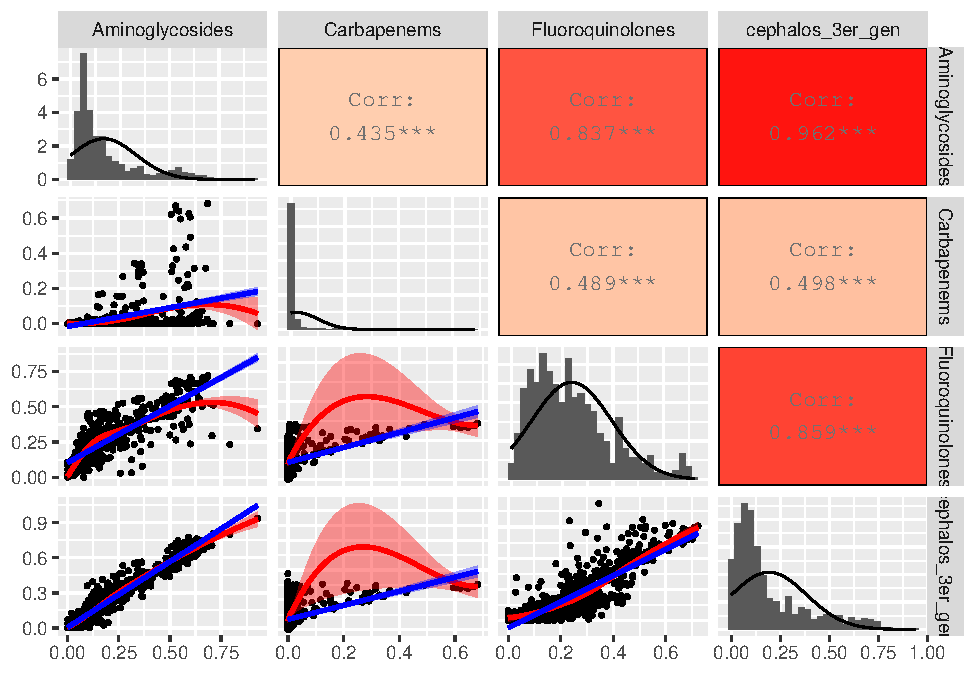
\includegraphics{1_actividad_analisis_general_files/figure-latex/Código para diagrama de dispresión y correlaciones-1.pdf}
\caption{Gráfica de dispersión y correlaciones}
\end{figure}

El resultado de la figura 1. da información valiosa para el desarrollo
del resto de las actividades. En primera medida como se puede observar y
anticipar las variables de estudio no siguen una distribución normal, e
incluso es posible concluir que la variable \texttt{Carbapenems} es la
menos informativa ya que exhibe la menor correlación con las demás; en
las regresiones lineales realizadas entre variables (líneas azules:
método \texttt{lm} y rojas: metodo local \texttt{loess}, en las
dispersiones de la cuadricula inferior) se observa una pobre relación
lineal. Inclusive se evidencia poca dispersión de los datos de esta
variable. Esto indica que las bacterias estudiadas cuando son
resistentes a los Carbapenems, necesariamente no son resistentes a otros
antibióticos.

Diferente a lo observado para las cefalosporinas de 3er generación. Como
se puede observar en la figura 1. existe una alta correlación y relación
lineal entre la variables \texttt{Cephalos\_3er\_gen} y
\texttt{Aminoglycosides} (Corr = 0.962) y \texttt{Cephalos\_3er\_gen} y
\texttt{Fluoroquinolones} (Corr = 0.837). Lo que indica que cuando hay
resistencia a Cefalosporia de 3er generación también se espera que se de
resistencia a Aminoglicosidos y Fluoroquinolonas.

\hypertarget{b-diagrama-de-estrellas}{%
\paragraph{(b) diagrama de estrellas}\label{b-diagrama-de-estrellas}}

\begin{figure}
\centering
\includegraphics{1_actividad_analisis_general_files/figure-latex/Código para diagrama de estrellas-1.pdf}
\caption{Diagrama de estrellas para las variables estudiadas}
\end{figure}

La figura 2. muestra por cada observación el peso que tiene cada
variable a través de las proporciones mostradas en los segmentos que
conforman la estrella. Como se puede observar, aunque con la cantidad de
datos que se están estudiando es difícil visualizar el diagrama
adecuadamente, las observaciones donde el porcentaje de resistencia es
mayor (radio de la estrella mayor), se evidencia el poco peso de la
variable \texttt{Carbapenems} esto muy problemente está dado a la baja
resistencia encontrada para la mayor parte de las observaciones en este
estudio.

\hypertarget{c-caras-de-chernoff}{%
\paragraph{(c) caras de Chernoff}\label{c-caras-de-chernoff}}

Para elaborar este diagrama se realizó una selección al azar de 100
observaciones, esto con el fin de poder visualizar y especificar mejor
cada uno de los rasgos de la caras. Esta estratégia es poco eficiente
cuando la cantidad de datos es alta.

\begin{figure}
\centering
\includegraphics{1_actividad_analisis_general_files/figure-latex/Código para caras de Chernoff-1.pdf}
\caption{Diagrama de caras de Chernoff}
\end{figure}

\begin{verbatim}
## effect of variables:
##  modified item       Var               
##  "height of face   " "Aminoglycosides" 
##  "width of face    " "Carbapenems"     
##  "structure of face" "Fluoroquinolones"
##  "height of mouth  " "cephalos_3er_gen"
##  "width of mouth   " "Aminoglycosides" 
##  "smiling          " "Carbapenems"     
##  "height of eyes   " "Fluoroquinolones"
##  "width of eyes    " "cephalos_3er_gen"
##  "height of hair   " "Aminoglycosides" 
##  "width of hair   "  "Carbapenems"     
##  "style of hair   "  "Fluoroquinolones"
##  "height of nose  "  "cephalos_3er_gen"
##  "width of nose   "  "Aminoglycosides" 
##  "width of ear    "  "Carbapenems"     
##  "height of ear   "  "Fluoroquinolones"
\end{verbatim}

Como se puede ver en la figura 3. y la leyenda que la acompaña, a cada
variable se le asigna un conjunto de rasgos, y se evalua para cada una
de las observaciones el impacto que tiene cada variable. En este
análisis llama la atención la cara de la observación número 76, esta
cara es ancha y el pelo es ancho y de estilo particular; esto indica las
variables \texttt{Carbapenems} y \texttt{Fluoroquinolonas} (`width of
face' lo que corresponde a \texttt{Carbapenems}, `width of hair' que
corresponde también a \texttt{Carbapenems} y `style of hair' que
corresponde a \texttt{Fluoroquinolones}) son las más representativas en
esta observación.

\hypertarget{d-curvas-de-andrews}{%
\paragraph{(d) curvas de Andrews}\label{d-curvas-de-andrews}}

Para este gráfico se definió evaluar la consistencia y correlaciones de
las variables númericas dadas con relación a una variable categórica
\texttt{Year}. Se definió esta variable como \texttt{factor} y se
incluyo en el análisis.

\begin{figure}
\centering
\includegraphics{1_actividad_analisis_general_files/figure-latex/Código para curvas de Andrews-1.pdf}
\caption{Curvas de Andrew}
\end{figure}

En la figura 4. se observa que la dimesionalidad de las curvas
esparcialmente constante. Algunas se observaciones se comportan más
planas y otras más onduladas lo que corresponde a observaciones que
tiene dimensionalidades con relación al los años distintas al conjunto
de datos.

\hypertarget{e-otros-gruxe1ficos-apropiados}{%
\paragraph{(e) otros gráficos
apropiados}\label{e-otros-gruxe1ficos-apropiados}}

Además se eleaboraron gráficos tipo ``boxplots'' para cada una de las
variables que corresponden a los porcentajes de resistencia a
determinado antibiótico; esto se analizó por año, tipo de bacteria y
region.

\begin{figure}
\centering
\includegraphics{1_actividad_analisis_general_files/figure-latex/Código Boxplot 1-1.pdf}
\caption{Boxplot 1: resistencia a Aminoglucosidos por bacteria y region
en tiempo}
\end{figure}

El Boxplot 1. corresponde a al análisis de la resistencia de las dos
bacterias seleccionadas para este ejercicio (\emph{Escherichia coli;
Klebsiella pneumoniae}) al grupo de antibióticos conocido como
``aminoglucosidos''. Para este grupos evidencia un incremento leve de la
resistencia a los antbióticos de los dos tipos de bacteria en el tiempo.
La bacteria que exhibe mayores porcentajes y varianza en la resistencia
a los antibióticos es la \emph{Klebsiella pneumoniae}, esto es
particularmente relevante para las regiones del este y sur de europa
(Èastern\texttt{,}Southern`). Llama la atención que en estas regiones el
incremento de los resportes de resistencia a aminoglucosidos incremento
en el 2005, esto puede estar correlacionado con mayor reporte de niveles
de resistencia y mayor conciencia de la problemática mundial con
respecto a la resistencia a antibióticos.

\begin{figure}
\centering
\includegraphics{1_actividad_analisis_general_files/figure-latex/Código Boxplot 2-1.pdf}
\caption{Boxplot 2: resistencia a Carbapenems por bacteria y region en
tiempo}
\end{figure}

El Boxplot 2. que se encuentra gráficado en la figura 6. resulta
particularmente interesante, dado que muestra la baja frecuencia de
resistencia al grupo de antibióticos conocido como \texttt{Carbapenems}.
Al igual que con los Animoglucosidos, la bacteria que reporta mayor
resistencia es la \emph{Klebsiella pneumoniae} para las regiones de este
y sur de europa. En este caso el incremento de resistencia incia desde
el año 2009. Esta información, asociada a las correlaciones mostradas en
la figura 1. muestran el poco peso que tienen los Carbapenemicos en la
resistencia total a los antibióticos y la resistencia combinada.

\begin{figure}
\centering
\includegraphics{1_actividad_analisis_general_files/figure-latex/Código Boxplot 3-1.pdf}
\caption{Boxplots 3: resistencia a Fluoroquinolonas por bacteria y
region en tiempo}
\end{figure}

El boxplot número 4. representa el porcentaje de resistencia al grupo de
antibióticos ``Fluoroquinolonas''. Respecto a este grupo, se observa un
incremento en el tiempo de la resistencia en todas las regiones y para
las dos bacterias. Las regiones del occidente de europa \texttt{western}
se evidencia un incremento inicial y una estabilización de este
comportamiento desde el 2009. Las regiones de sur y este de europa se ve
el mayor incremento y variabilidad en la resistencia especialmente en la
bacteria \emph{Klebsiella pneumoniae}, desde el 2005. Que al igual a los
casos anteriores puede estar dada al incremento y frecuencia del
reporte.

\begin{figure}
\centering
\includegraphics{1_actividad_analisis_general_files/figure-latex/Código Boxplot 4-1.pdf}
\caption{Boxplot 4: resistencia a Cefalosporinas de 3 generación por
bacteria y region en tiempo}
\end{figure}

Finalmente la figura 8 muestra la resistencia a las ceaflosporinas de
3er generación. Para estas el incremento de la resistencia presenta un
incremento sostenido en el tiempo. De la misma forma la bacteria
\emph{Klebsiella pneumoniae} es la que presenta mayores niveles y
variabilidad de la resistencia, especialmente en la región del sur y
este de europa, siendo mayor en esta última desde el 2005.

\hypertarget{cuarta-pregunta}{%
\subsubsection{Cuarta pregunta:}\label{cuarta-pregunta}}

\begin{quote}
Investigue si su conjunto de datos proviene de una distribución normal
multivariada.
\end{quote}

Para comprar la normalidad de los datos se decidió comprobar a través de
un test de Shapiro-Wilk multivariado, el cual permite constatar la
normalidad del conjunto de observaciones, y se formula de la siguiente
manera (donde \(N\) indica una distribución normal:

\[
H_o: el\ conjunto \ de\ datos = N
\]

\[
H_1: el\ conjunto \ de\ datos \neq N 
\]

\begin{longtable}[]{@{}cc@{}}
\caption{Test de shapiro-wilk (w) para los datos}\tabularnewline
\toprule
\begin{minipage}[b]{0.10\columnwidth}\centering
\(W\)\strut
\end{minipage} & \begin{minipage}[b]{0.16\columnwidth}\centering
\(p-value\)\strut
\end{minipage}\tabularnewline
\midrule
\endfirsthead
\toprule
\begin{minipage}[b]{0.10\columnwidth}\centering
\(W\)\strut
\end{minipage} & \begin{minipage}[b]{0.16\columnwidth}\centering
\(p-value\)\strut
\end{minipage}\tabularnewline
\midrule
\endhead
\begin{minipage}[t]{0.10\columnwidth}\centering
0.469\strut
\end{minipage} & \begin{minipage}[t]{0.16\columnwidth}\centering
2.489e-44\strut
\end{minipage}\tabularnewline
\bottomrule
\end{longtable}

El resultado obtenido de este estadístico es presentado en la tabla 5.
lo que arroja un valor de \(W =0.469\) significativo
(\(p - value < 0.05\)), por tal razón, se rechaza la hipotesis nula, así
que se puede aseverar los datos no siguen una distribución normal
(\(N\)).

\end{document}
